\documentclass{article}

% if you need to pass options to natbib, use, e.g.:
% \PassOptionsToPackage{numbers, compress}{natbib}
% before loading nips_2016
%
% to avoid loading the natbib package, add option nonatbib:
% \usepackage[nonatbib]{nips_2016}

\usepackage[nonatbib,final]{nips_2016}

% to compile a camera-ready version, add the [final] option, e.g.:
% \usepackage[final]{nips_2016}

\usepackage[utf8]{inputenc} % allow utf-8 input
\usepackage[T1]{fontenc}    % use 8-bit T1 fonts
\usepackage{hyperref}       % hyperlinks
\usepackage{url}            % simple URL typesetting
\usepackage{booktabs}       % professional-quality tables
\usepackage{amsfonts}       % blackboard math symbols
\usepackage{nicefrac}       % compact symbols for 1/2, etc.
\usepackage{microtype}      % microtypography
\usepackage{physics}		 % Physics package for derivatives
\usepackage{graphicx,float,caption,subcaption,tikz}
\usepackage{listings}
\usepackage{color} %red, green, blue, yellow, cyan, magenta, black, white
\usepackage{animate}
\usepackage{multirow}
\usepackage{pgffor}
\usepackage{tabularx}

\usepackage{amsmath}
\usepackage{latexsym}
\usepackage{amssymb}
\usepackage{mathtools}
\usepackage{bm}
\usepackage{array}
\captionsetup[table]{skip=10pt}

\DeclareMathOperator*{\argmax}{\arg\max}
\DeclareMathOperator*{\argmin}{\arg\min}
\DeclareMathOperator*{\E}{\mathbb{E}}

\usepackage[backend=bibtex,sorting=none,autocite=superscript]{biblatex}

\DeclareCiteCommand{\supercite}[\mkbibsuperscript]
  {\iffieldundef{prenote}
     {}
     {\BibliographyWarning{Ignoring prenote argument}}%
   \iffieldundef{postnote}
     {}
     {\BibliographyWarning{Ignoring postnote argument}}}
  {\usebibmacro{citeindex}%
   \bibopenbracket\usebibmacro{cite}\bibclosebracket}
  {\supercitedelim}
  {}
  
\bibliography{references}
\let\cite=\supercite
\graphicspath{ {results/} }

\newcounter{codenum}
\newcounter{imgnum}
\makeatletter
\newtoks\@tabtoks
\newcommand\addtabtoks[1]{\global\@tabtoks\expandafter{\the\@tabtoks#1}}
\newcommand\eaddtabtoks[1]{\edef\mytmp{#1}\expandafter\addtabtoks\expandafter{\mytmp}}
\newcommand*\resettabtoks{\global\@tabtoks{}}
\newcommand*\printtabtoks{\the\@tabtoks}
\makeatother

\title{Computer Vision Report: Text to Image Synthesis}

% The \author macro works with any number of authors. There are two
% commands used to separate the names and addresses of multiple
% authors: \And and \AND.
%
% Using \And between authors leaves it to LaTeX to determine where to
% break the lines. Using \AND forces a line break at that point. So,
% if LaTeX puts 3 of 4 authors names on the first line, and the last
% on the second line, try using \AND instead of \And before the third
% author name.

\author{
  Ankit Vani \\
  \texttt{ankit.vani@nyu.edu} \\
  \And
  Srivas Venkatesh \\
  \texttt{srivas.venkatesh@nyu.edu} \\
}

\begin{document}

\maketitle

\begin{abstract}
  Generation of realistic images given a text describing it is a challenging and interesting problem. With the recent successes of Generative Adversarial Networks in this field, we aim to explore it and use information theoretical extension to it to isolate meaningful latent variables.
\end{abstract}

\section{Overview}

\subsection{DCGAN}

GAN:
\begin{align}
\min_G \max_D\, V(D,G) = \E_{x \sim p_{\text{data}}(x)}\left[\log D(x)\right] + \E_{z\sim p_z(z)}\left[\log(1-D(G(z)))\right] \label{eq:gan}
\end{align}


\subsection{Generative Adversarial Text to Image Synthesis}



Text to Image GAN:
\begin{align}
\min_G \max_D\, \mathcal{V}(D,G, \varphi) =& \E_{(x,t) \sim p_{\text{data}}(x,t)}\left[\log D(x, \varphi(t))\right]\, + \nonumber\\
&\E_{z\sim p_z(z), t\sim p_{\text{intdata}}(t)}\left[\log(1-D(G(z, \varphi(t)), \varphi(t)))\right] \label{eq:t2i}
\end{align}
where $t \sim p_{\text{intdata}}(t)$ is short for sampling as $t_1 \sim p_{\text{data}}(t), t_2 \sim p_{\text{data}}(t), \beta \sim [0,1], t = \beta t_1 + (1-\beta) t_2$.


\subsection{InfoGAN}

Mutual information
\begin{align}
\mathcal{I}(c;G(z,c)) = \mathcal{H}(G(z,c)) - \mathcal{H}(G(z,c) \mid c) = \mathcal{H}(c) - \mathcal{H}(c\mid G(z,c))
\end{align}

Variational lower bound
\begin{align}
\mathcal{I}(c;G(z,c)) &\geq \E_{x\sim G(z,c)}\left[\E_{c'\sim p(c\mid x)}\left[\log Q(c'\mid x)\right]\right] + \mathcal{H}(c)
\end{align}

or in our case
\begin{align}
\mathcal{I}(c;G(z,c,\varphi(t))) &\geq \E_{t\sim p_{\text{intdata}}(t), x\sim G(z,c,\varphi(t))}\left[\E_{c'\sim p(c\mid x,t)}\left[\log Q(c'\mid x,t)\right]\right] + \mathcal{H}(c)
\end{align}

Under suitable regularity conditions, we have the variational lower bound
\begin{align}
\mathcal{I}(c;G(z,c, \varphi(t))) &\geq \E_{c\sim p(c), t\sim p_{\text{intdata}}(t), x\sim G(z,c, \varphi(t))}\left[\log Q(c\mid x,t)\right] + \mathcal{H}(c) = \mathcal{L}_I(G,Q,\varphi) \label{eq:t2imiloss}
\end{align}

An alternate model is possible where we assume that the output of $Q$ is conditionally independent of $t$ given $x$, in which case $Q(c\mid x,t)$ simplifies to $Q(c\mid x)$. Equivalent to removing a direct edge between $t$ and $c'$ in the graphical model.

Text to Image InfoGAN:
\begin{align}
\min_{G,Q} \max_D\, \mathcal{V}_{\text{InfoGAN}}(D,G,Q,\varphi) = \mathcal{V}(D,G,\varphi) - \lambda \mathcal{L}_I(G,Q,\varphi)
\end{align}
where $\mathcal{V}(D,G,\varphi)$ from Equation (\ref{eq:t2i}), $\mathcal{L}_I(G,Q,\varphi)$ from Equation (\ref{eq:t2imiloss}).




\section{Our Approach}

\section{Code Used}

\section{Experimental Results}
\begin{table}[H]
\begin{tabularx}{\textwidth}{|c|X|X|X|X|X|X|X|X|X|X|}
\hline
Latent Code & 1 & 2 & 3 & 4 & 5 & 6 & 7 & 8 & 9 & 10\\
\hline
%\multirow{5}{\hsize}{this vibrant red bird has a pointed black beak}
%\foreach \code in {1,...,5}{
%    \eaddtabtoks{\code}
%    \foreach \img in {1,...,10}{
%        \eaddtabtoks{& \includegraphics{cub_5c_l01_txt_btch2/img_1_\code_\img}}
%    }
%    \addtabtoks{\\\hline}
%}
%\printtabtoks
%\resettabtoks
1 & 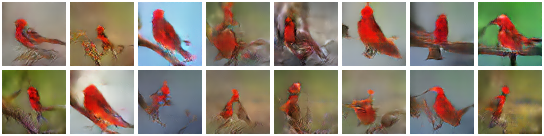
\includegraphics[keepaspectratio,height=50px]{cub_5c_l01_txt_btch2/img_1_1_1} & 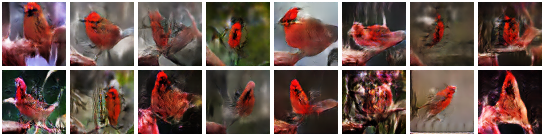
\includegraphics[keepaspectratio,height=50px]{cub_5c_l01_txt_btch2/img_1_1_2} & 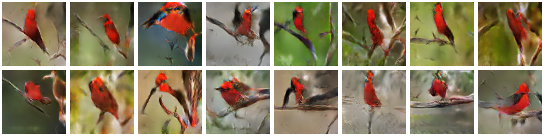
\includegraphics[keepaspectratio,height=50px]{cub_5c_l01_txt_btch2/img_1_1_3} & 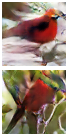
\includegraphics[keepaspectratio,height=50px]{cub_5c_l01_txt_btch2/img_1_1_4} & 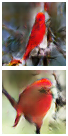
\includegraphics[keepaspectratio,height=50px]{cub_5c_l01_txt_btch2/img_1_1_5} & 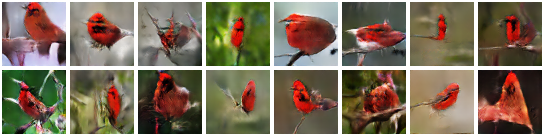
\includegraphics[keepaspectratio,height=50px]{cub_5c_l01_txt_btch2/img_1_1_6} & 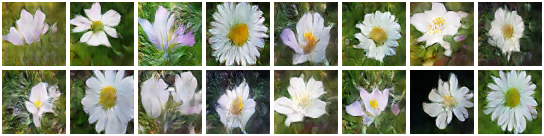
\includegraphics[keepaspectratio,height=50px]{cub_5c_l01_txt_btch2/img_1_1_7} & 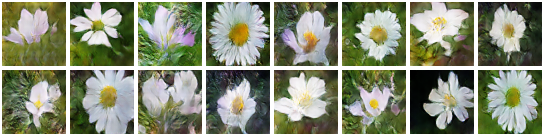
\includegraphics[keepaspectratio,height=50px]{cub_5c_l01_txt_btch2/img_1_1_8} & 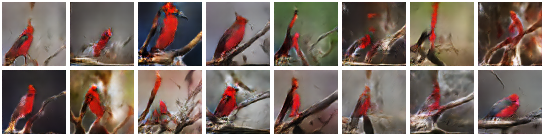
\includegraphics[keepaspectratio,height=50px]{cub_5c_l01_txt_btch2/img_1_1_9} & 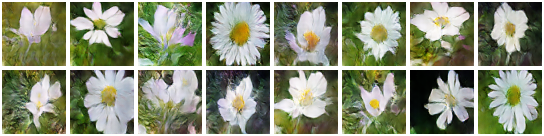
\includegraphics[keepaspectratio,height=50px]{cub_5c_l01_txt_btch2/img_1_1_10} \\\hline
2 & 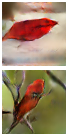
\includegraphics[keepaspectratio,height=50px]{cub_5c_l01_txt_btch2/img_1_2_1} & 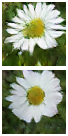
\includegraphics[keepaspectratio,height=50px]{cub_5c_l01_txt_btch2/img_1_2_2} & 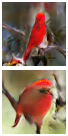
\includegraphics[keepaspectratio,height=50px]{cub_5c_l01_txt_btch2/img_1_2_3} & 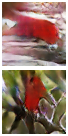
\includegraphics[keepaspectratio,height=50px]{cub_5c_l01_txt_btch2/img_1_2_4} & 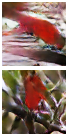
\includegraphics[keepaspectratio,height=50px]{cub_5c_l01_txt_btch2/img_1_2_5} & 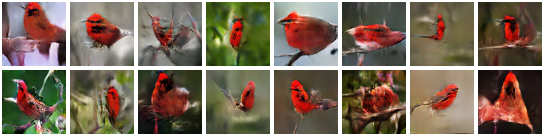
\includegraphics[keepaspectratio,height=50px]{cub_5c_l01_txt_btch2/img_1_2_6} & 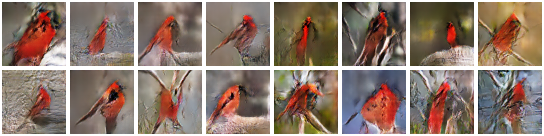
\includegraphics[keepaspectratio,height=50px]{cub_5c_l01_txt_btch2/img_1_2_7} & 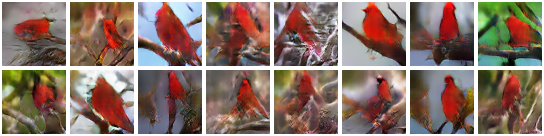
\includegraphics[keepaspectratio,height=50px]{cub_5c_l01_txt_btch2/img_1_2_8} & 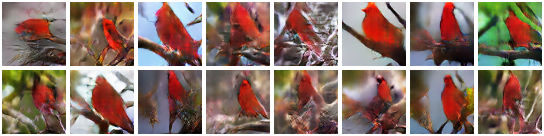
\includegraphics[keepaspectratio,height=50px]{cub_5c_l01_txt_btch2/img_1_2_9} & 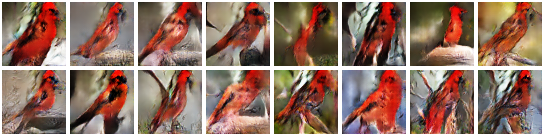
\includegraphics[keepaspectratio,height=50px]{cub_5c_l01_txt_btch2/img_1_2_10} \\\hline
3 & 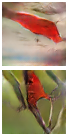
\includegraphics[keepaspectratio,height=50px]{cub_5c_l01_txt_btch2/img_1_3_1} & 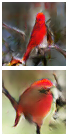
\includegraphics[keepaspectratio,height=50px]{cub_5c_l01_txt_btch2/img_1_3_2} & 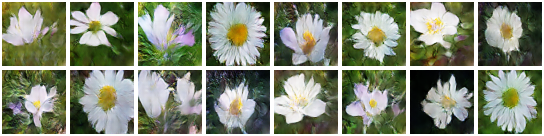
\includegraphics[keepaspectratio,height=50px]{cub_5c_l01_txt_btch2/img_1_3_3} & 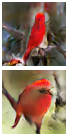
\includegraphics[keepaspectratio,height=50px]{cub_5c_l01_txt_btch2/img_1_3_4} & 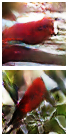
\includegraphics[keepaspectratio,height=50px]{cub_5c_l01_txt_btch2/img_1_3_5} & 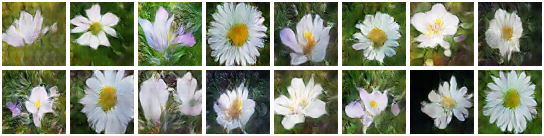
\includegraphics[keepaspectratio,height=50px]{cub_5c_l01_txt_btch2/img_1_3_6} & 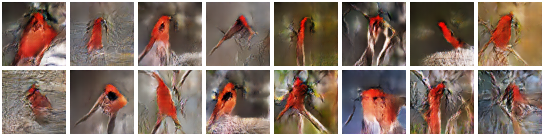
\includegraphics[keepaspectratio,height=50px]{cub_5c_l01_txt_btch2/img_1_3_7} & 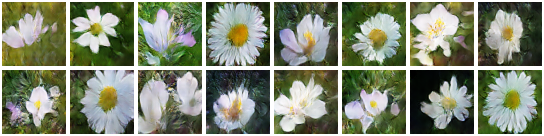
\includegraphics[keepaspectratio,height=50px]{cub_5c_l01_txt_btch2/img_1_3_8} & 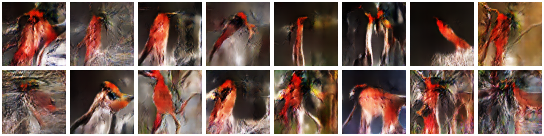
\includegraphics[keepaspectratio,height=50px]{cub_5c_l01_txt_btch2/img_1_3_9} & 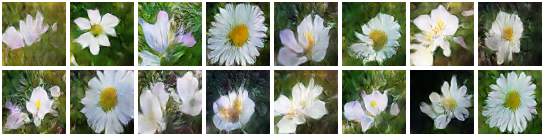
\includegraphics[keepaspectratio,height=50px]{cub_5c_l01_txt_btch2/img_1_3_10} \\\hline
4 & 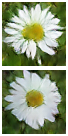
\includegraphics[keepaspectratio,height=50px]{cub_5c_l01_txt_btch2/img_1_4_1} & 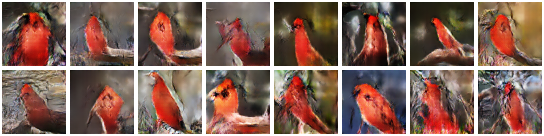
\includegraphics[keepaspectratio,height=50px]{cub_5c_l01_txt_btch2/img_1_4_2} & 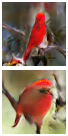
\includegraphics[keepaspectratio,height=50px]{cub_5c_l01_txt_btch2/img_1_4_3} & 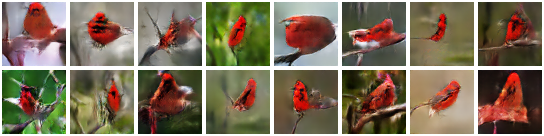
\includegraphics[keepaspectratio,height=50px]{cub_5c_l01_txt_btch2/img_1_4_4} & 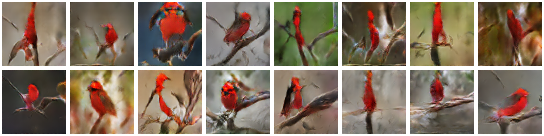
\includegraphics[keepaspectratio,height=50px]{cub_5c_l01_txt_btch2/img_1_4_5} & 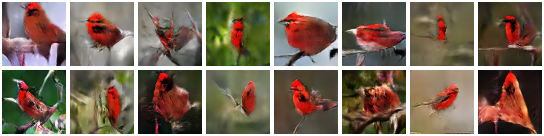
\includegraphics[keepaspectratio,height=50px]{cub_5c_l01_txt_btch2/img_1_4_6} & 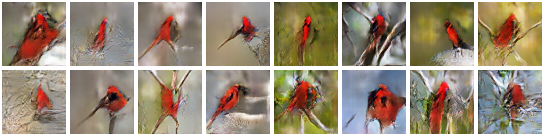
\includegraphics[keepaspectratio,height=50px]{cub_5c_l01_txt_btch2/img_1_4_7} & 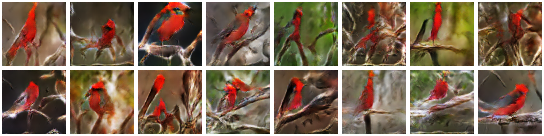
\includegraphics[keepaspectratio,height=50px]{cub_5c_l01_txt_btch2/img_1_4_8} & 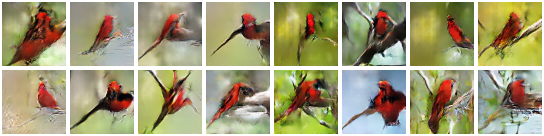
\includegraphics[keepaspectratio,height=50px]{cub_5c_l01_txt_btch2/img_1_4_9} & 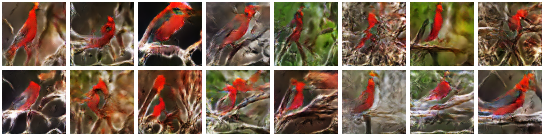
\includegraphics[keepaspectratio,height=50px]{cub_5c_l01_txt_btch2/img_1_4_10} \\\hline
5 & 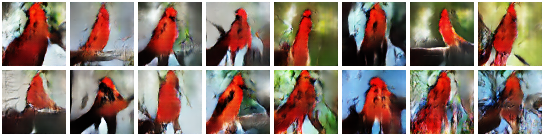
\includegraphics[keepaspectratio,height=50px]{cub_5c_l01_txt_btch2/img_1_5_1} & 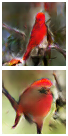
\includegraphics[keepaspectratio,height=50px]{cub_5c_l01_txt_btch2/img_1_5_2} & 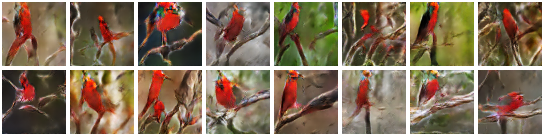
\includegraphics[keepaspectratio,height=50px]{cub_5c_l01_txt_btch2/img_1_5_3} & 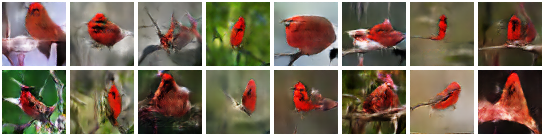
\includegraphics[keepaspectratio,height=50px]{cub_5c_l01_txt_btch2/img_1_5_4} & 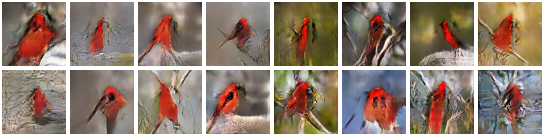
\includegraphics[keepaspectratio,height=50px]{cub_5c_l01_txt_btch2/img_1_5_5} & 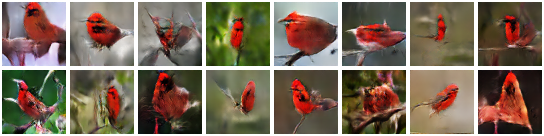
\includegraphics[keepaspectratio,height=50px]{cub_5c_l01_txt_btch2/img_1_5_6} & 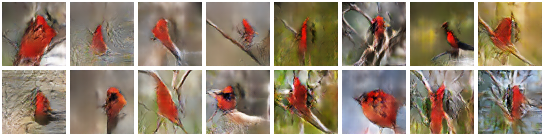
\includegraphics[keepaspectratio,height=50px]{cub_5c_l01_txt_btch2/img_1_5_7} & 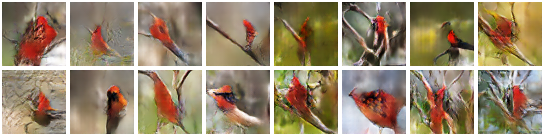
\includegraphics[keepaspectratio,height=50px]{cub_5c_l01_txt_btch2/img_1_5_8} & 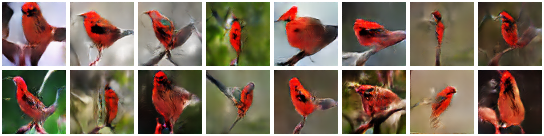
\includegraphics[keepaspectratio,height=50px]{cub_5c_l01_txt_btch2/img_1_5_9} & \includegraphics[keepaspectratio,height=50px]{cub_5c_l01_txt_btch2/img_1_5_10} \\\hline
\end{tabularx}
\end{table}

\begin{table}[H]
\begin{tabularx}{\textwidth}{|c|X|X|X|X|X|X|X|X|X|X|}
\hline
Latent Code & 1 & 2 & 3 & 4 & 5 & 6 & 7 & 8 & 9 & 10\\
\hline
1 & \includegraphics[keepaspectratio,height=50px]{cub_3c_2d_l01_txt_btch2/img_1_1_1} & \includegraphics[keepaspectratio,height=50px]{cub_3c_2d_l01_txt_btch2/img_1_1_2} & \includegraphics[keepaspectratio,height=50px]{cub_3c_2d_l01_txt_btch2/img_1_1_3} & \includegraphics[keepaspectratio,height=50px]{cub_3c_2d_l01_txt_btch2/img_1_1_4} & \includegraphics[keepaspectratio,height=50px]{cub_3c_2d_l01_txt_btch2/img_1_1_5} & \includegraphics[keepaspectratio,height=50px]{cub_3c_2d_l01_txt_btch2/img_1_1_6} & \includegraphics[keepaspectratio,height=50px]{cub_3c_2d_l01_txt_btch2/img_1_1_7} & \includegraphics[keepaspectratio,height=50px]{cub_3c_2d_l01_txt_btch2/img_1_1_8} & \includegraphics[keepaspectratio,height=50px]{cub_3c_2d_l01_txt_btch2/img_1_1_9} & \includegraphics[keepaspectratio,height=50px]{cub_3c_2d_l01_txt_btch2/img_1_1_10} \\\hline
2 & \includegraphics[keepaspectratio,height=50px]{cub_3c_2d_l01_txt_btch2/img_1_2_1} & \includegraphics[keepaspectratio,height=50px]{cub_3c_2d_l01_txt_btch2/img_1_2_2} & \includegraphics[keepaspectratio,height=50px]{cub_3c_2d_l01_txt_btch2/img_1_2_3} & \includegraphics[keepaspectratio,height=50px]{cub_3c_2d_l01_txt_btch2/img_1_2_4} & \includegraphics[keepaspectratio,height=50px]{cub_3c_2d_l01_txt_btch2/img_1_2_5} & \includegraphics[keepaspectratio,height=50px]{cub_3c_2d_l01_txt_btch2/img_1_2_6} & \includegraphics[keepaspectratio,height=50px]{cub_3c_2d_l01_txt_btch2/img_1_2_7} & \includegraphics[keepaspectratio,height=50px]{cub_3c_2d_l01_txt_btch2/img_1_2_8} & \includegraphics[keepaspectratio,height=50px]{cub_3c_2d_l01_txt_btch2/img_1_2_9} & \includegraphics[keepaspectratio,height=50px]{cub_3c_2d_l01_txt_btch2/img_1_2_10} \\\hline
3 & \includegraphics[keepaspectratio,height=50px]{cub_3c_2d_l01_txt_btch2/img_1_3_1} & \includegraphics[keepaspectratio,height=50px]{cub_3c_2d_l01_txt_btch2/img_1_3_2} & \includegraphics[keepaspectratio,height=50px]{cub_3c_2d_l01_txt_btch2/img_1_3_3} & \includegraphics[keepaspectratio,height=50px]{cub_3c_2d_l01_txt_btch2/img_1_3_4} & \includegraphics[keepaspectratio,height=50px]{cub_3c_2d_l01_txt_btch2/img_1_3_5} & \includegraphics[keepaspectratio,height=50px]{cub_3c_2d_l01_txt_btch2/img_1_3_6} & \includegraphics[keepaspectratio,height=50px]{cub_3c_2d_l01_txt_btch2/img_1_3_7} & \includegraphics[keepaspectratio,height=50px]{cub_3c_2d_l01_txt_btch2/img_1_3_8} & \includegraphics[keepaspectratio,height=50px]{cub_3c_2d_l01_txt_btch2/img_1_3_9} & \includegraphics[keepaspectratio,height=50px]{cub_3c_2d_l01_txt_btch2/img_1_3_10} \\\hline
\end{tabularx}
\end{table}
%\animategraphics[loop,controls,autoplay]{12}{cub_5c_l01_notxt/img_1_3_}{1}{10}
\section{Conclusion}

\printbibliography

\end{document}
